%!TEX root = pset2.tex

\section{Logistic Regression}\label{sec:lr}

\subsection{Implementation}
We implemented $L_2$-regularized logistic regression using gradient descent. The objective function to be minimized over is:
\begin{equation}
\sum_{i=1}^n \log (1 + e^{-y^{(i)}(\M w^T\M x^{(i)} + w_0)}) + \lambda \M w^T\M w
\end{equation}

We used both our implementation of gradient descend and the \texttt{Matlab} function \texttt{fminunc}. Convergence criterion is reached within reasonable iterations in both implementations.

\subsection{Testing in data with $\lambda = 0$}
We run the logistic regression on the four data sets, setting the regularization parameter $\lambda = 0$. The estimated coefficients are listed in Table \ref{tab:LR_reg_coeff}.

\begin{table}[h!]
\centering
\caption{Estimated logistic regression coefficients and accuracy, $\lambda = 0$ }
\begin{tabular}{lrrrrr}
  \hline\hline
  Data   & $w_0$ 	& $w_1$ 	  & $w_2$ 	& Training accuracy & Validation accuracy\\
  \hline
  stdev1 & -66.3378  & 95.2461 & 101.1527 & 1.0000    & 1.0000    \\
  stdev2 & -0.0466   & 0.7636  & 1.1148 	& 0.9075    & 0.9200    \\
  stdev4 & -0.0093   & 0.2363  & 0.2034 	& 0.7400    & 0.7525    \\
  nonsep & 0.0006    & -0.0247 & -0.0237	& 0.5150    & 0.4925\\
  \hline\hline
\end{tabular}\label{tab:LR_reg_coeff}
\end{table}

The decision boundaries at various thresholds are plotted in Figure \ref{fig:LR_plots}. We observe the following phenomenon:
\begin{enumerate}
\item As data become more linearly non-separable, the accuracy is lower, and the decision boundary has higher variance with respect to data (for example, as $\sigma$ increases, the decision boundary and accuracy are more different between training and validation.)
\item As data become more linearly non-separable, the estimated logistic function is also less steep, reflected in the wider bands in the plots and lower norm of $\M w$. This is reasonable because the classifier is not as certain about how to classify the data points in the mix zone.
\item In the totally non-separable case, logistic regression fails to classify, barely reaching the $50\%$ baseline.
\end{enumerate}


\begin{figure}[h!]
\centering
    \begin{subfigure}[b]{0.4\textwidth}
	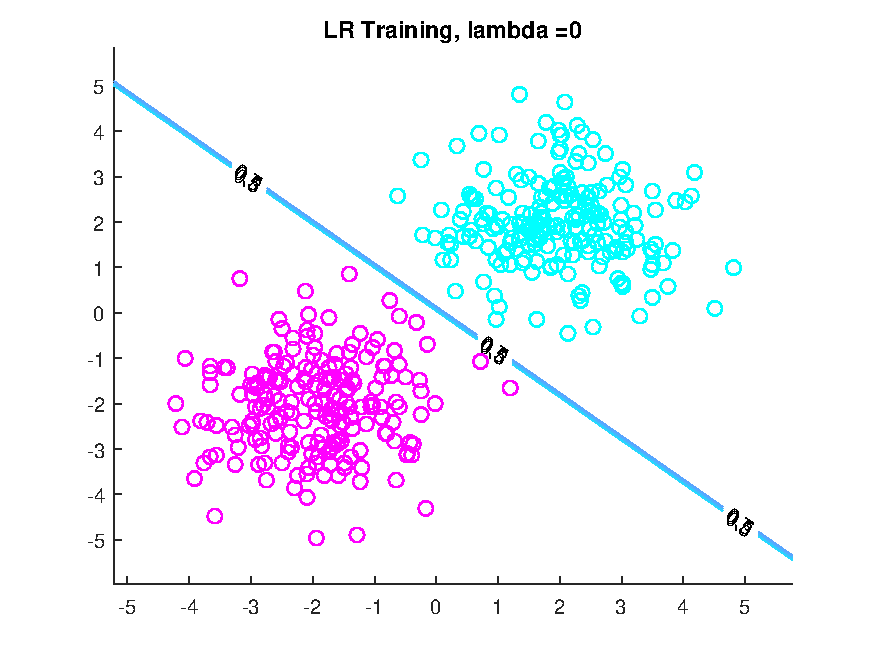
\includegraphics[scale=0.4]{hw2_1_stdev1_a_0.pdf}
	\caption{Data with $\sigma = 1$, training}\label{fig:data_stdev1a}
    \end{subfigure}
    \quad
    \begin{subfigure}[b]{0.4\textwidth}
	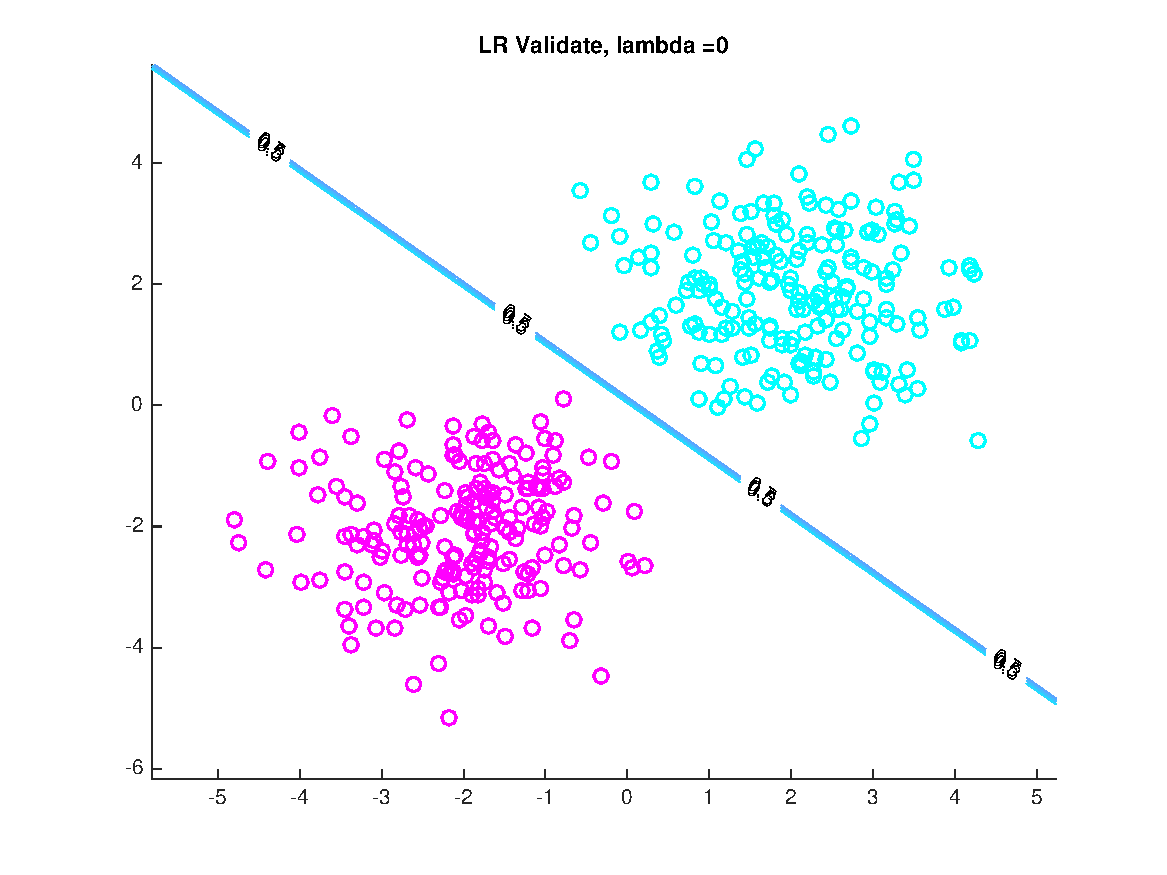
\includegraphics[scale=0.4]{hw2_1_stdev1_b_0.pdf}
	\caption{Data with $\sigma = 1$, validation}\label{fig:data_stdev1b}
    \end{subfigure}

    \begin{subfigure}[b]{0.4\textwidth}
	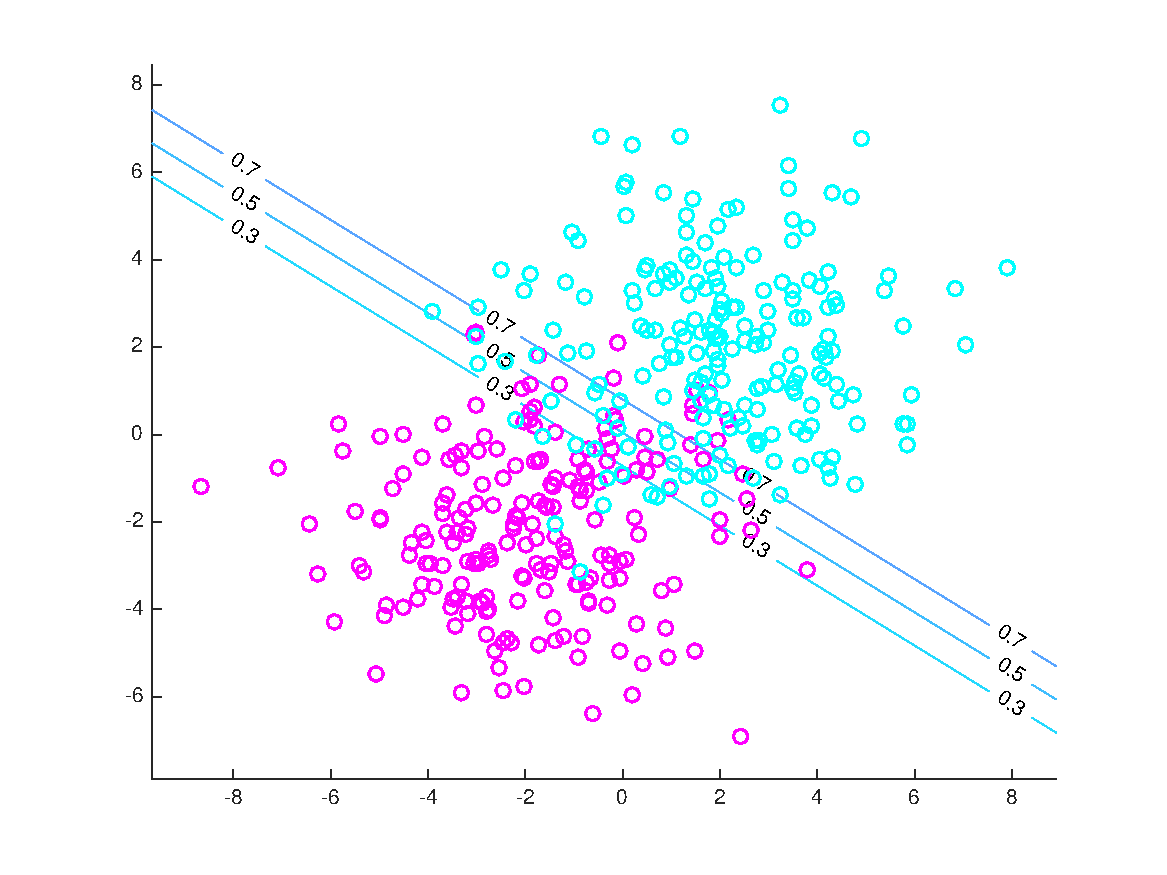
\includegraphics[scale=0.4]{hw2_1_stdev2_a_0.pdf}
	\caption{Data with $\sigma = 2$, training}\label{fig:data_stdev2a}
	\end{subfigure}
	\quad	
	\begin{subfigure}[b]{0.4\textwidth}
	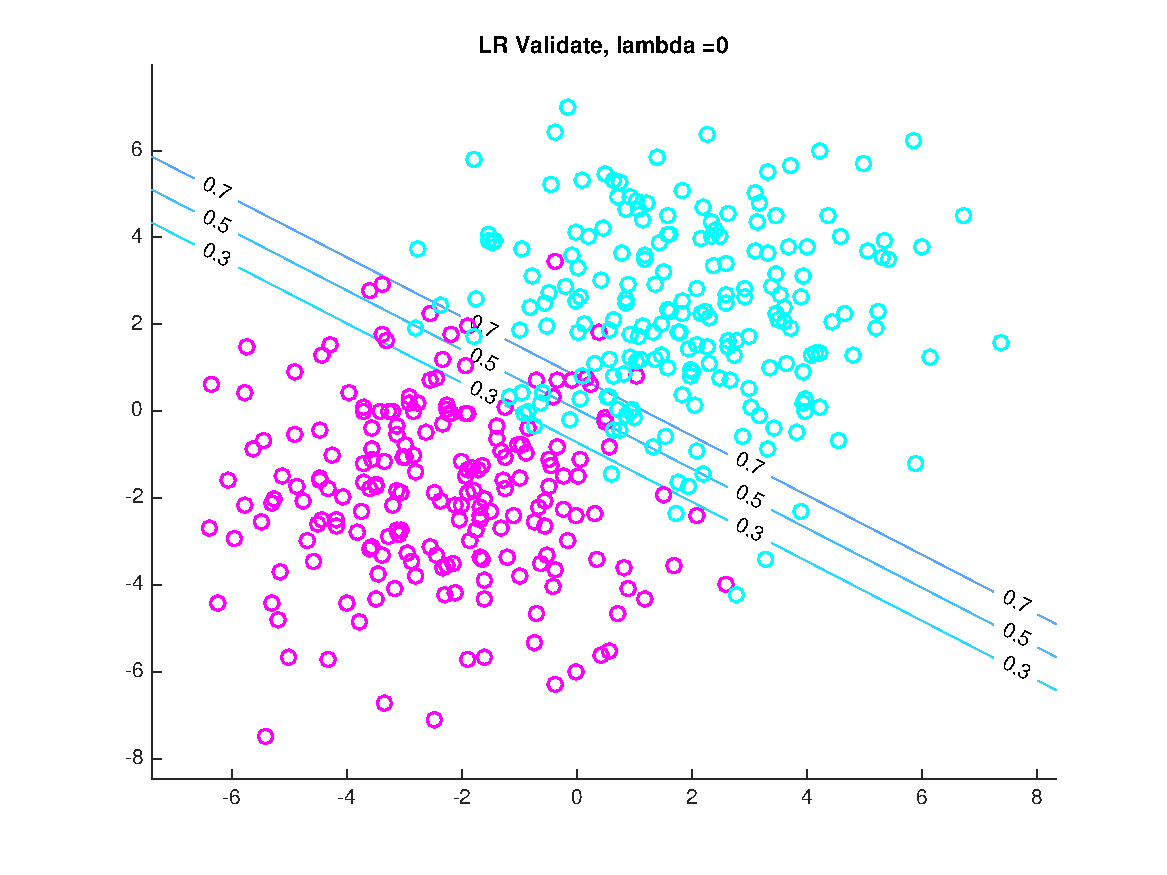
\includegraphics[scale=0.4]{hw2_1_stdev2_b_0.pdf}
	\caption{Data with $\sigma = 2$, validation}\label{fig:data_stdev2b}
	\end{subfigure}
    
    \begin{subfigure}[b]{0.4\textwidth}
	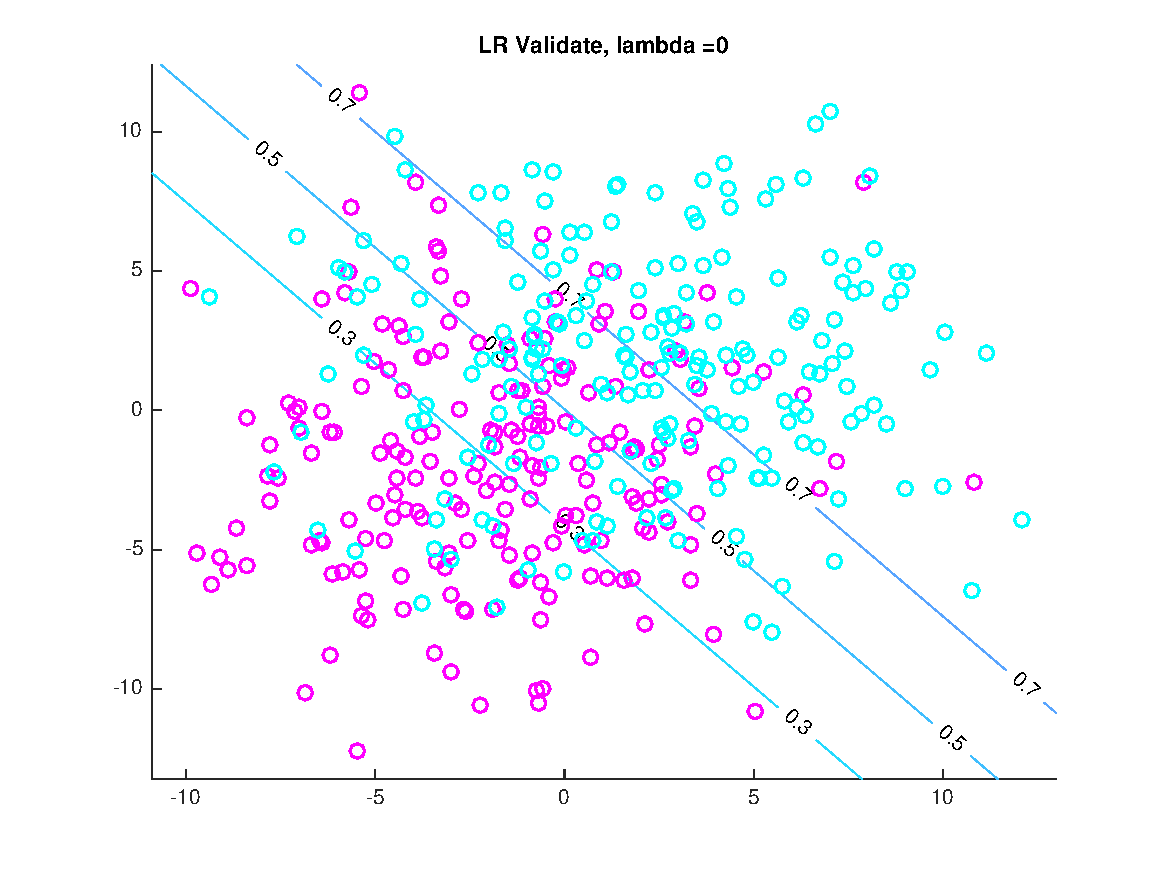
\includegraphics[scale=0.4]{hw2_1_stdev4_a_0.pdf}
	\caption{Data with $\sigma = 4$, training}\label{fig:data_stdev4a}
    \end{subfigure}  
    \quad
    \begin{subfigure}[b]{0.4\textwidth}
	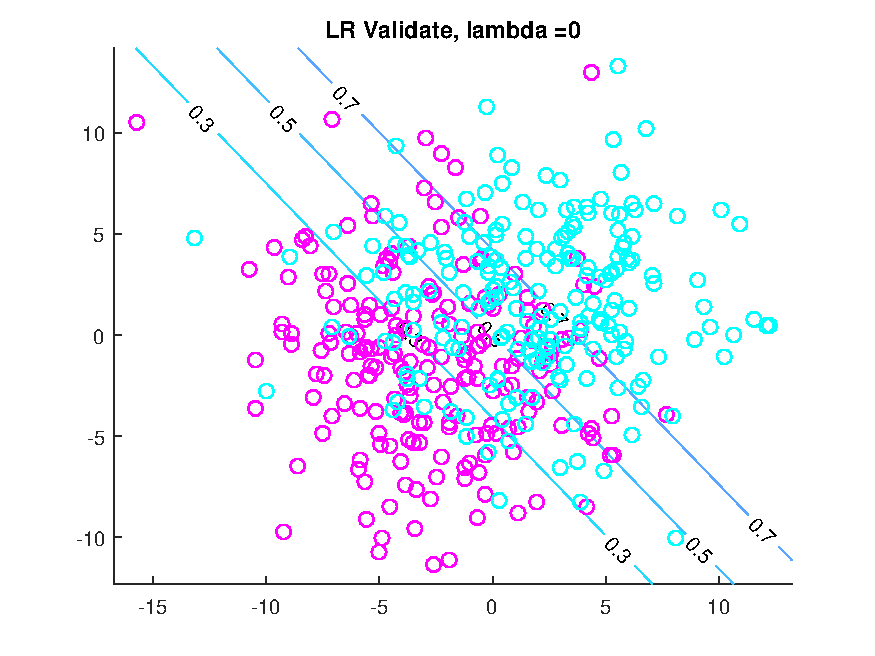
\includegraphics[scale=0.4]{hw2_1_stdev4_b_0.pdf}
	\caption{Data with $\sigma = 4$, validation}\label{fig:data_stdev4b}
    \end{subfigure}  

    \begin{subfigure}[b]{0.4\textwidth}
	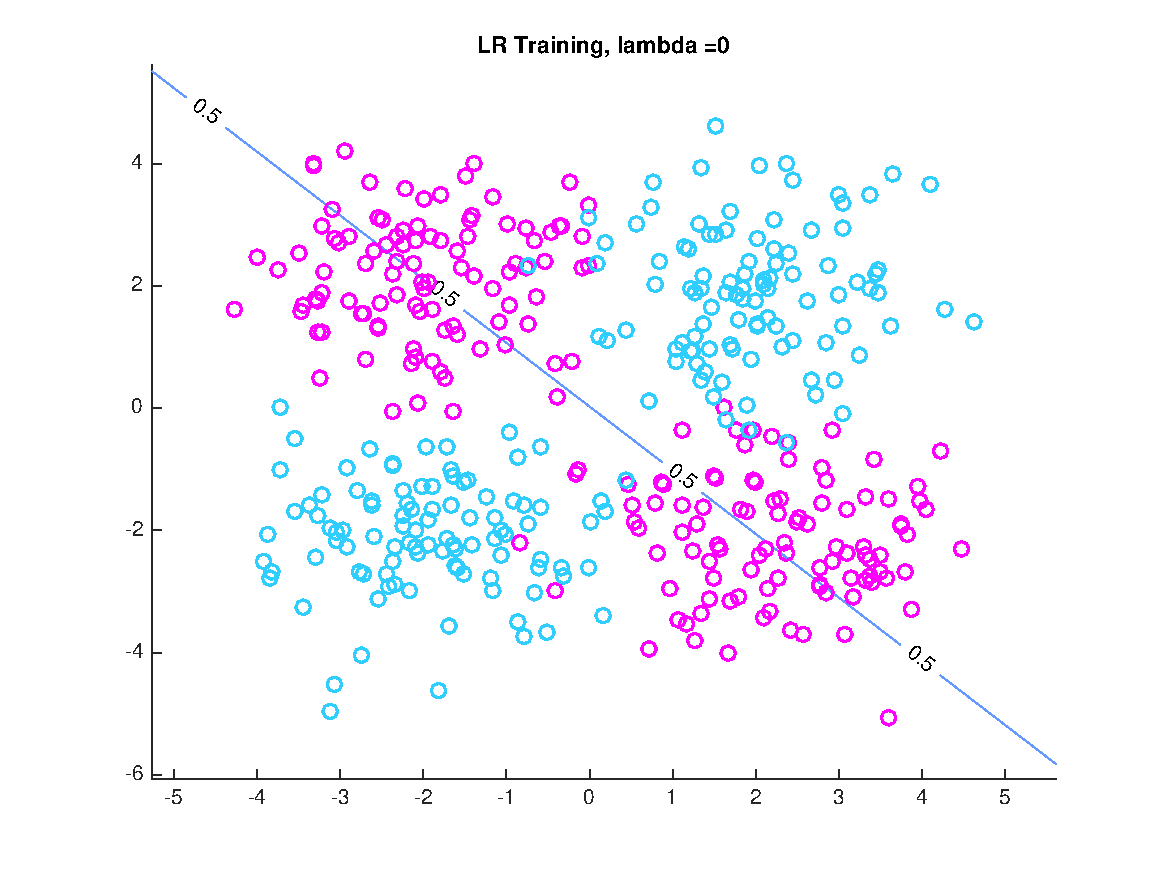
\includegraphics[scale=0.4]{hw2_1_nonsep_a_0.pdf}
	\caption{Non-seperable data, training}\label{fig:data_nonsep_a}
    \end{subfigure}  
    \quad
    \begin{subfigure}[b]{0.4\textwidth}
	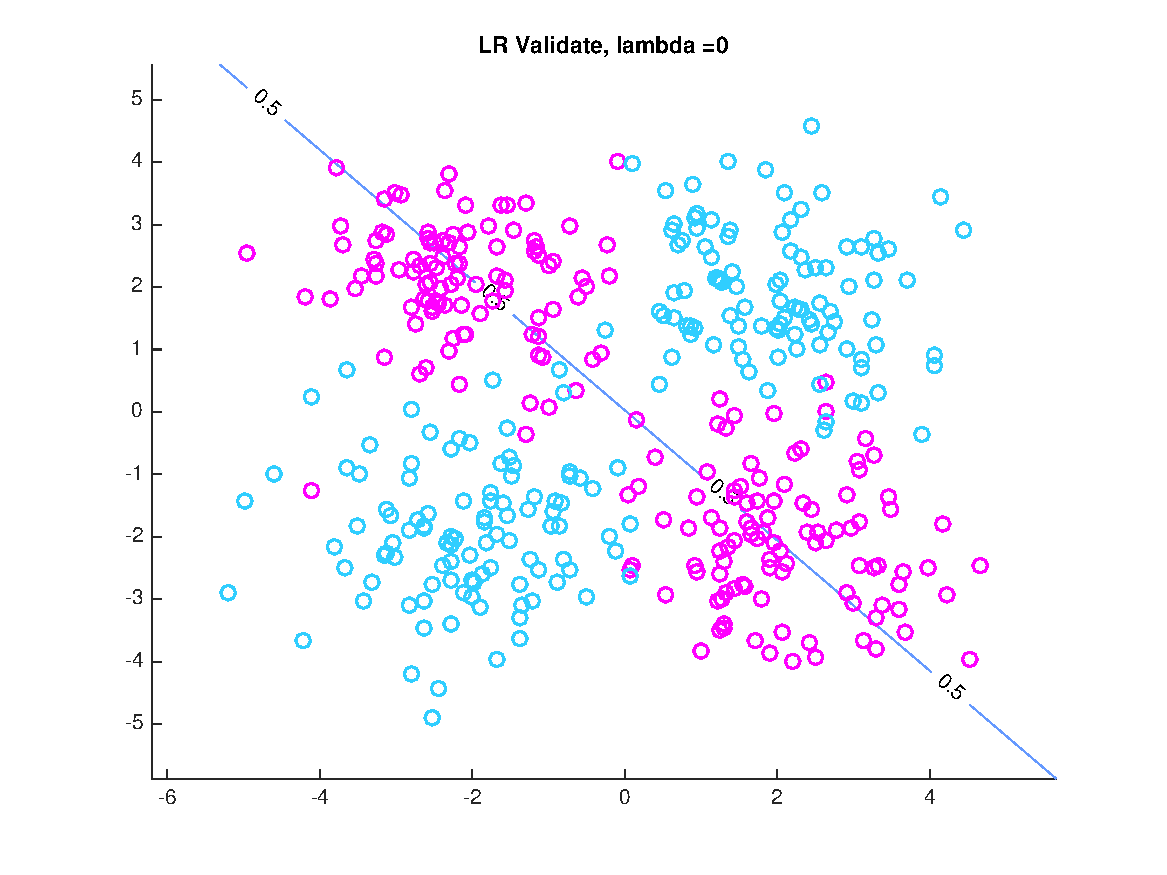
\includegraphics[scale=0.4]{hw2_1_nonsep_b_0.pdf}
	\caption{Non-seperable data, validation}\label{fig:data_nonsep_b}
    \end{subfigure}  
    \caption{Plots of decision boundaries from logistic regression with various $\lambda$ and data sets.}  \label{fig:LR_plots}  
\end{figure}


\subsection{Testing in data with positive $\lambda$}
Similarly, we run logistic regression with other values of $\lambda$. In particular, we use the cross-validation technique to select best value of $\lambda$ using the validation set accuracy. In particular, for the four datasets, we choose $\lambda = 0$, $\lambda = 0$, $\lambda = 100$, and $\lambda = 1000$ respectively.